\documentclass[1p]{elsarticle_modified}
%\bibliographystyle{elsarticle-num}

%\usepackage[colorlinks]{hyperref}
%\usepackage{abbrmath_seonhwa} %\Abb, \Ascr, \Acal ,\Abf, \Afrak
\usepackage{amsfonts}
\usepackage{amssymb}
\usepackage{amsmath}
\usepackage{amsthm}
\usepackage{scalefnt}
\usepackage{amsbsy}
\usepackage{kotex}
\usepackage{caption}
\usepackage{subfig}
\usepackage{color}
\usepackage{graphicx}
\usepackage{xcolor} %% white, black, red, green, blue, cyan, magenta, yellow
\usepackage{float}
\usepackage{setspace}
\usepackage{hyperref}

\usepackage{tikz}
\usetikzlibrary{arrows}

\usepackage{multirow}
\usepackage{array} % fixed length table
\usepackage{hhline}

%%%%%%%%%%%%%%%%%%%%%
\makeatletter
\renewcommand*\env@matrix[1][\arraystretch]{%
	\edef\arraystretch{#1}%
	\hskip -\arraycolsep
	\let\@ifnextchar\new@ifnextchar
	\array{*\c@MaxMatrixCols c}}
\makeatother %https://tex.stackexchange.com/questions/14071/how-can-i-increase-the-line-spacing-in-a-matrix
%%%%%%%%%%%%%%%

\usepackage[normalem]{ulem}

\newcommand{\msout}[1]{\ifmmode\text{\sout{\ensuremath{#1}}}\else\sout{#1}\fi}
%SOURCE: \msout is \stkout macro in https://tex.stackexchange.com/questions/20609/strikeout-in-math-mode

\newcommand{\cancel}[1]{
	\ifmmode
	{\color{red}\msout{#1}}
	\else
	{\color{red}\sout{#1}}
	\fi
}

\newcommand{\add}[1]{
	{\color{blue}\uwave{#1}}
}

\newcommand{\replace}[2]{
	\ifmmode
	{\color{red}\msout{#1}}{\color{blue}\uwave{#2}}
	\else
	{\color{red}\sout{#1}}{\color{blue}\uwave{#2}}
	\fi
}

\newcommand{\Sol}{\mathcal{S}} %segment
\newcommand{\D}{D} %diagram
\newcommand{\A}{\mathcal{A}} %arc


%%%%%%%%%%%%%%%%%%%%%%%%%%%%%5 test

\def\sl{\operatorname{\textup{SL}}(2,\Cbb)}
\def\psl{\operatorname{\textup{PSL}}(2,\Cbb)}
\def\quan{\mkern 1mu \triangleright \mkern 1mu}

\theoremstyle{definition}
\newtheorem{thm}{Theorem}[section]
\newtheorem{prop}[thm]{Proposition}
\newtheorem{lem}[thm]{Lemma}
\newtheorem{ques}[thm]{Question}
\newtheorem{cor}[thm]{Corollary}
\newtheorem{defn}[thm]{Definition}
\newtheorem{exam}[thm]{Example}
\newtheorem{rmk}[thm]{Remark}
\newtheorem{alg}[thm]{Algorithm}

\newcommand{\I}{\sqrt{-1}}
\begin{document}

%\begin{frontmatter}
%
%\title{Boundary parabolic representations of knots up to 8 crossings}
%
%%% Group authors per affiliation:
%\author{Yunhi Cho} 
%\address{Department of Mathematics, University of Seoul, Seoul, Korea}
%\ead{yhcho@uos.ac.kr}
%
%
%\author{Seonhwa Kim} %\fnref{s_kim}}
%\address{Center for Geometry and Physics, Institute for Basic Science, Pohang, 37673, Korea}
%\ead{ryeona17@ibs.re.kr}
%
%\author{Hyuk Kim}
%\address{Department of Mathematical Sciences, Seoul National University, Seoul 08826, Korea}
%\ead{hyukkim@snu.ac.kr}
%
%\author{Seokbeom Yoon}
%\address{Department of Mathematical Sciences, Seoul National University, Seoul, 08826,  Korea}
%\ead{sbyoon15@snu.ac.kr}
%
%\begin{abstract}
%We find all boundary parabolic representation of knots up to 8 crossings.
%
%\end{abstract}
%\begin{keyword}
%    \MSC[2010] 57M25 
%\end{keyword}
%
%\end{frontmatter}

%\linenumbers
%\tableofcontents
%
\newcommand\colored[1]{\textcolor{white}{\rule[-0.35ex]{0.8em}{1.4ex}}\kern-0.8em\color{red} #1}%
%\newcommand\colored[1]{\textcolor{white}{ #1}\kern-2.17ex	\textcolor{white}{ #1}\kern-1.81ex	\textcolor{white}{ #1}\kern-2.15ex\color{red}#1	}

{\Large $\underline{12n_{0148}~(K12n_{0148})}$}

\setlength{\tabcolsep}{10pt}
\renewcommand{\arraystretch}{1.6}
\vspace{1cm}\begin{tabular}{m{100pt}>{\centering\arraybackslash}m{274pt}}
\multirow{5}{120pt}{
	\centering
	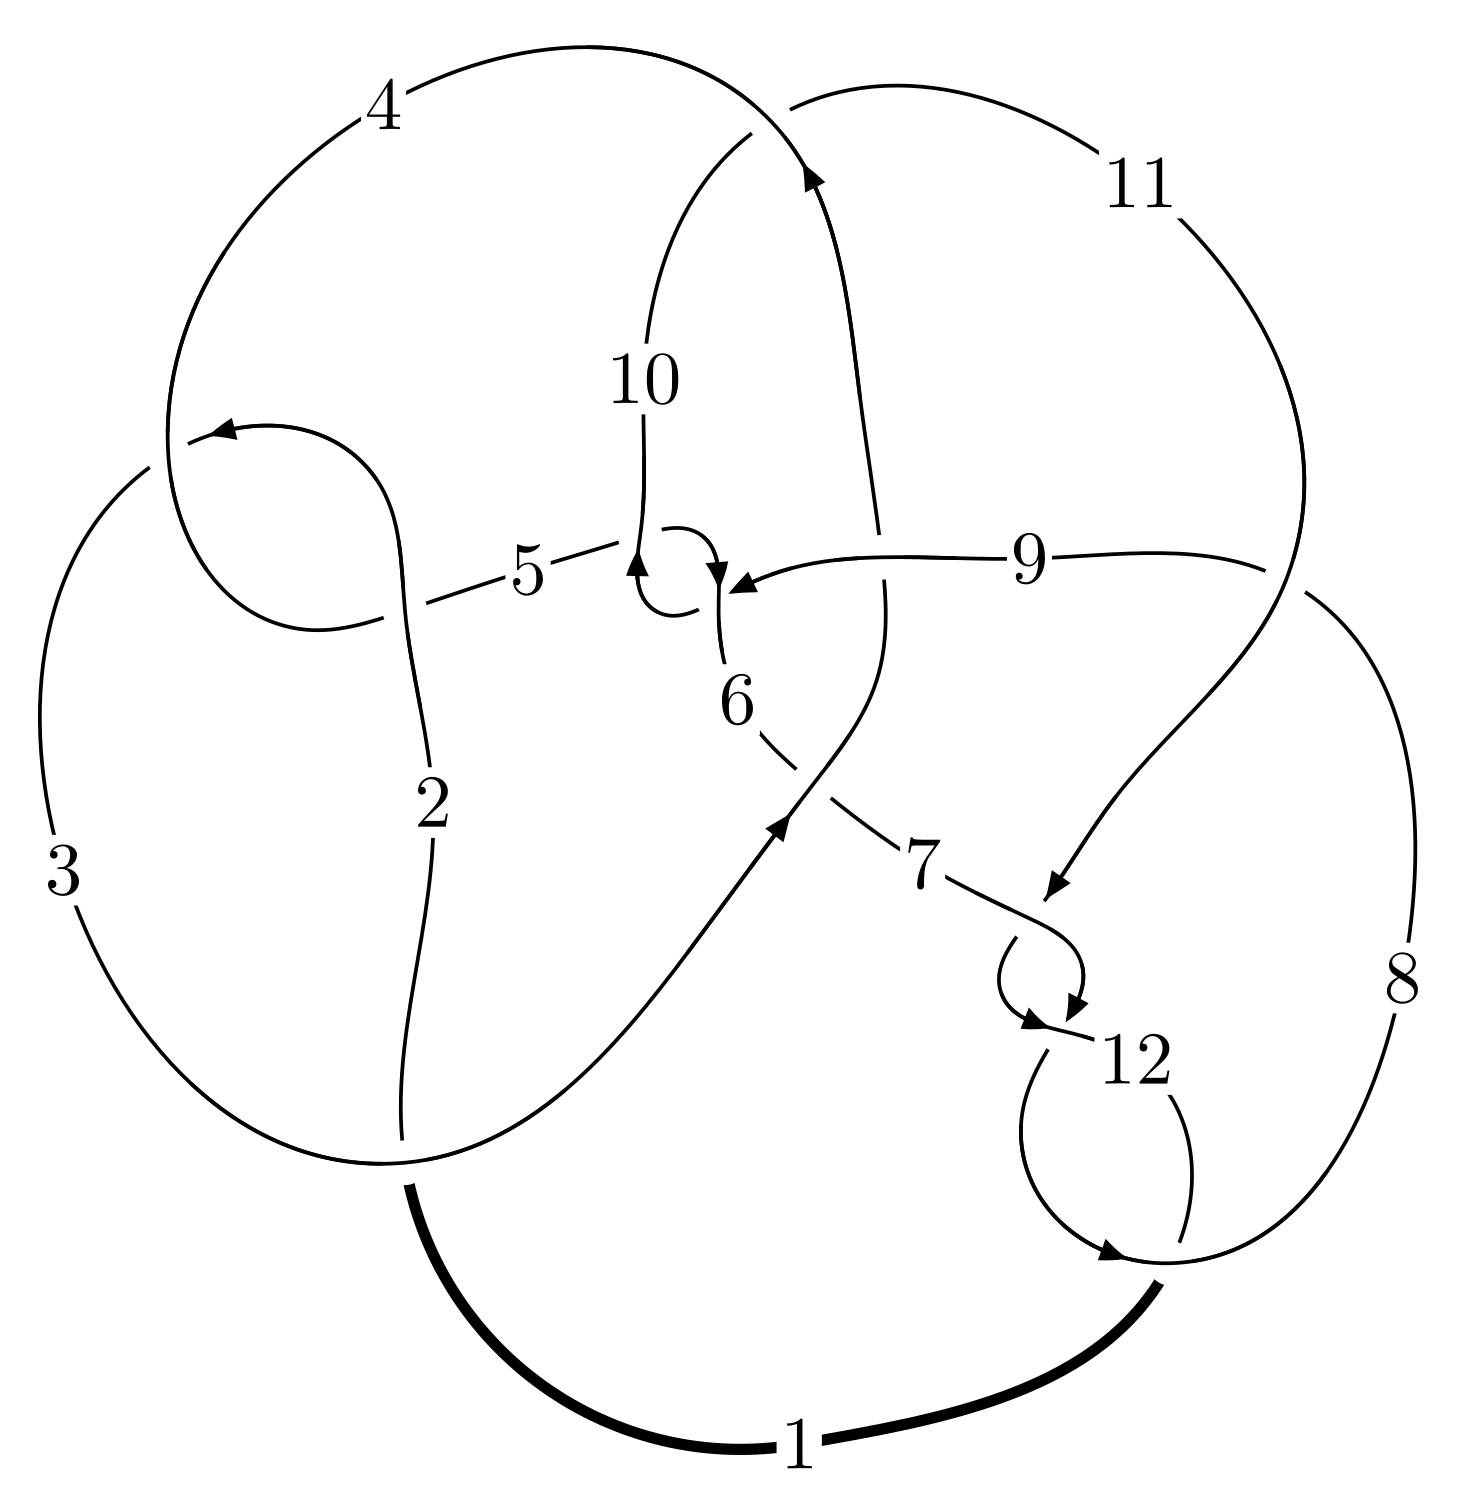
\includegraphics[width=112pt]{../../../GIT/diagram.site/Diagrams/png/2237_12n_0148.png}\\
\ \ \ A knot diagram\footnotemark}&
\allowdisplaybreaks
\textbf{Linearized knot diagam} \\
\cline{2-2}
 &
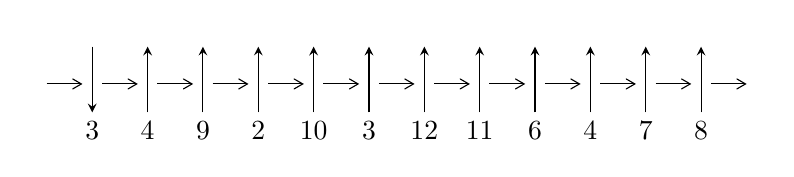
\begin{tikzpicture}[x=20pt, y=17pt]
	% nodes
	\node (C0) at (0, 0) {};
	\node (C1) at (1, 0) {};
	\node (C1U) at (1, +1) {};
	\node (C1D) at (1, -1) {3};

	\node (C2) at (2, 0) {};
	\node (C2U) at (2, +1) {};
	\node (C2D) at (2, -1) {4};

	\node (C3) at (3, 0) {};
	\node (C3U) at (3, +1) {};
	\node (C3D) at (3, -1) {9};

	\node (C4) at (4, 0) {};
	\node (C4U) at (4, +1) {};
	\node (C4D) at (4, -1) {2};

	\node (C5) at (5, 0) {};
	\node (C5U) at (5, +1) {};
	\node (C5D) at (5, -1) {10};

	\node (C6) at (6, 0) {};
	\node (C6U) at (6, +1) {};
	\node (C6D) at (6, -1) {3};

	\node (C7) at (7, 0) {};
	\node (C7U) at (7, +1) {};
	\node (C7D) at (7, -1) {12};

	\node (C8) at (8, 0) {};
	\node (C8U) at (8, +1) {};
	\node (C8D) at (8, -1) {11};

	\node (C9) at (9, 0) {};
	\node (C9U) at (9, +1) {};
	\node (C9D) at (9, -1) {6};

	\node (C10) at (10, 0) {};
	\node (C10U) at (10, +1) {};
	\node (C10D) at (10, -1) {4};

	\node (C11) at (11, 0) {};
	\node (C11U) at (11, +1) {};
	\node (C11D) at (11, -1) {7};

	\node (C12) at (12, 0) {};
	\node (C12U) at (12, +1) {};
	\node (C12D) at (12, -1) {8};
	\node (C13) at (13, 0) {};

	% arrows
	\draw[->,>={angle 60}]
	(C0) edge (C1) (C1) edge (C2) (C2) edge (C3) (C3) edge (C4) (C4) edge (C5) (C5) edge (C6) (C6) edge (C7) (C7) edge (C8) (C8) edge (C9) (C9) edge (C10) (C10) edge (C11) (C11) edge (C12) (C12) edge (C13) ;	\draw[->,>=stealth]
	(C1U) edge (C1D) (C2D) edge (C2U) (C3D) edge (C3U) (C4D) edge (C4U) (C5D) edge (C5U) (C6D) edge (C6U) (C7D) edge (C7U) (C8D) edge (C8U) (C9D) edge (C9U) (C10D) edge (C10U) (C11D) edge (C11U) (C12D) edge (C12U) ;
	\end{tikzpicture} \\
\hhline{~~} \\& 
\textbf{Solving Sequence} \\ \cline{2-2} 
 &
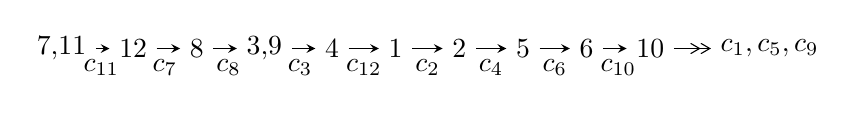
\begin{tikzpicture}[x=23pt, y=7pt]
	% node
	\node (A0) at (-1/8, 0) {7,11};
	\node (A1) at (1, 0) {12};
	\node (A2) at (2, 0) {8};
	\node (A3) at (49/16, 0) {3,9};
	\node (A4) at (33/8, 0) {4};
	\node (A5) at (41/8, 0) {1};
	\node (A6) at (49/8, 0) {2};
	\node (A7) at (57/8, 0) {5};
	\node (A8) at (65/8, 0) {6};
	\node (A9) at (73/8, 0) {10};
	\node (C1) at (1/2, -1) {$c_{11}$};
	\node (C2) at (3/2, -1) {$c_{7}$};
	\node (C3) at (5/2, -1) {$c_{8}$};
	\node (C4) at (29/8, -1) {$c_{3}$};
	\node (C5) at (37/8, -1) {$c_{12}$};
	\node (C6) at (45/8, -1) {$c_{2}$};
	\node (C7) at (53/8, -1) {$c_{4}$};
	\node (C8) at (61/8, -1) {$c_{6}$};
	\node (C9) at (69/8, -1) {$c_{10}$};
	\node (A10) at (11, 0) {$c_{1},c_{5},c_{9}$};

	% edge
	\draw[->,>=stealth]	
	(A0) edge (A1) (A1) edge (A2) (A2) edge (A3) (A3) edge (A4) (A4) edge (A5) (A5) edge (A6) (A6) edge (A7) (A7) edge (A8) (A8) edge (A9) ;
	\draw[->>,>={angle 60}]	
	(A9) edge (A10);
\end{tikzpicture} \\ 

\end{tabular} \\

\footnotetext{
The image of knot diagram is generated by the software ``\textbf{Draw programme}" developed by Andrew Bartholomew(\url{http://www.layer8.co.uk/maths/draw/index.htm\#Running-draw}), where we modified some parts for our purpose(\url{https://github.com/CATsTAILs/LinksPainter}).
}\phantom \\ \newline 
\centering \textbf{Ideals for irreducible components\footnotemark of $X_{\text{par}}$} 
 
\begin{align*}
I^u_{1}&=\langle 
5402057 u^{19}-3583441 u^{18}+\cdots+1977478 b+13308358,\\
\phantom{I^u_{1}}&\phantom{= \langle  }-639093 u^{19}+2151139 u^{18}+\cdots+1977478 a-11355740,\;u^{20}- u^{19}+\cdots+8 u-1\rangle \\
I^u_{2}&=\langle 
u^5 a+2 u^4 a-4 u^3 a-5 u^4-3 u^2 a+a u+10 u^2+5 b-3 a,\\
\phantom{I^u_{2}}&\phantom{= \langle  }u^5 a-2 u^5-3 u^3 a+u^2 a+6 u^3+a^2+2 a u+u^2- a-6 u-1,\;u^6-3 u^4+2 u^2+1\rangle \\
\\
\end{align*}
\raggedright * 2 irreducible components of $\dim_{\mathbb{C}}=0$, with total 32 representations.\\
\footnotetext{All coefficients of polynomials are rational numbers. But the coefficients are sometimes approximated in decimal forms when there is not enough margin.}
\newpage
\renewcommand{\arraystretch}{1}
\centering \section*{I. $I^u_{1}= \langle 5.40\times10^{6} u^{19}-3.58\times10^{6} u^{18}+\cdots+1.98\times10^{6} b+1.33\times10^{7},\;-6.39\times10^{5} u^{19}+2.15\times10^{6} u^{18}+\cdots+1.98\times10^{6} a-1.14\times10^{7},\;u^{20}- u^{19}+\cdots+8 u-1 \rangle$}
\flushleft \textbf{(i) Arc colorings}\\
\begin{tabular}{m{7pt} m{180pt} m{7pt} m{180pt} }
\flushright $a_{7}=$&$\begin{pmatrix}0\\u\end{pmatrix}$ \\
\flushright $a_{11}=$&$\begin{pmatrix}1\\0\end{pmatrix}$ \\
\flushright $a_{12}=$&$\begin{pmatrix}1\\- u^2\end{pmatrix}$ \\
\flushright $a_{8}=$&$\begin{pmatrix}u\\- u^3+u\end{pmatrix}$ \\
\flushright $a_{3}=$&$\begin{pmatrix}0.323186 u^{19}-1.08782 u^{18}+\cdots-21.2507 u+5.74254\\-2.73179 u^{19}+1.81213 u^{18}+\cdots+39.4687 u-6.72997\end{pmatrix}$ \\
\flushright $a_{9}=$&$\begin{pmatrix}- u^3+2 u\\- u^3+u\end{pmatrix}$ \\
\flushright $a_{4}=$&$\begin{pmatrix}-0.119500 u^{19}-0.378541 u^{18}+\cdots-7.19615 u+2.43256\\-3.10782 u^{19}+2.21574 u^{18}+\cdots+47.4853 u-8.50446\end{pmatrix}$ \\
\flushright $a_{1}=$&$\begin{pmatrix}- u^2+1\\u^4-2 u^2\end{pmatrix}$ \\
\flushright $a_{2}=$&$\begin{pmatrix}2.81060 u^{19}-2.56427 u^{18}+\cdots-52.8262 u+10.8039\\-3.18615 u^{19}+1.40304 u^{18}+\cdots+33.4356 u-4.59062\end{pmatrix}$ \\
\flushright $a_{5}=$&$\begin{pmatrix}4.68409 u^{19}-2.27049 u^{18}+\cdots-53.3439 u+8.58394\\1.97808 u^{19}-0.907299 u^{18}+\cdots-22.6536 u+3.12055\end{pmatrix}$ \\
\flushright $a_{6}=$&$\begin{pmatrix}-3.69057 u^{19}+2.49256 u^{18}+\cdots+52.9545 u-9.28098\\1.03914 u^{19}-0.150948 u^{18}+\cdots-5.14484 u+0.559226\end{pmatrix}$ \\
\flushright $a_{10}=$&$\begin{pmatrix}-2.78422 u^{19}+0.960462 u^{18}+\cdots+26.8596 u-3.11259\\-2.92442 u^{19}+1.93725 u^{18}+\cdots+42.5149 u-7.01762\end{pmatrix}$\\&\end{tabular}
\flushleft \textbf{(ii) Obstruction class $= -1$}\\~\\
\flushleft \textbf{(iii) Cusp Shapes $= \frac{8158475}{988739} u^{19}-\frac{7089886}{988739} u^{18}+\cdots-\frac{162706955}{988739} u+\frac{47565543}{988739}$}\\~\\
\newpage\renewcommand{\arraystretch}{1}
\flushleft \textbf{(iv) u-Polynomials at the component}\newline \\
\begin{tabular}{m{50pt}|m{274pt}}
Crossings & \hspace{64pt}u-Polynomials at each crossing \\
\hline $$\begin{aligned}c_{1}\end{aligned}$$&$\begin{aligned}
&u^{20}+43 u^{19}+\cdots-20046 u+625
\end{aligned}$\\
\hline $$\begin{aligned}c_{2},c_{4}\end{aligned}$$&$\begin{aligned}
&u^{20}- u^{19}+\cdots-214 u+25
\end{aligned}$\\
\hline $$\begin{aligned}c_{3}\end{aligned}$$&$\begin{aligned}
&u^{20}- u^{19}+\cdots+18 u-5
\end{aligned}$\\
\hline $$\begin{aligned}c_{5},c_{9}\end{aligned}$$&$\begin{aligned}
&u^{20}- u^{19}+\cdots+4 u-1
\end{aligned}$\\
\hline $$\begin{aligned}c_{6}\end{aligned}$$&$\begin{aligned}
&u^{20}+3 u^{19}+\cdots-70 u+1
\end{aligned}$\\
\hline $$\begin{aligned}c_{7},c_{11},c_{12}\end{aligned}$$&$\begin{aligned}
&u^{20}- u^{19}+\cdots+8 u-1
\end{aligned}$\\
\hline $$\begin{aligned}c_{8}\end{aligned}$$&$\begin{aligned}
&u^{20}+3 u^{19}+\cdots-162 u+17
\end{aligned}$\\
\hline $$\begin{aligned}c_{10}\end{aligned}$$&$\begin{aligned}
&u^{20}- u^{19}+\cdots-564 u-2209
\end{aligned}$\\
\hline
\end{tabular}\\~\\
\newpage\renewcommand{\arraystretch}{1}
\flushleft \textbf{(v) Riley Polynomials at the component}\newline \\
\begin{tabular}{m{50pt}|m{274pt}}
Crossings & \hspace{64pt}Riley Polynomials at each crossing \\
\hline $$\begin{aligned}c_{1}\end{aligned}$$&$\begin{aligned}
&y^{20}-253 y^{19}+\cdots-251953366 y+390625
\end{aligned}$\\
\hline $$\begin{aligned}c_{2},c_{4}\end{aligned}$$&$\begin{aligned}
&y^{20}+43 y^{19}+\cdots-20046 y+625
\end{aligned}$\\
\hline $$\begin{aligned}c_{3}\end{aligned}$$&$\begin{aligned}
&y^{20}- y^{19}+\cdots-214 y+25
\end{aligned}$\\
\hline $$\begin{aligned}c_{5},c_{9}\end{aligned}$$&$\begin{aligned}
&y^{20}+41 y^{19}+\cdots+84 y+1
\end{aligned}$\\
\hline $$\begin{aligned}c_{6}\end{aligned}$$&$\begin{aligned}
&y^{20}+49 y^{19}+\cdots-2266 y+1
\end{aligned}$\\
\hline $$\begin{aligned}c_{7},c_{11},c_{12}\end{aligned}$$&$\begin{aligned}
&y^{20}-15 y^{19}+\cdots-16 y+1
\end{aligned}$\\
\hline $$\begin{aligned}c_{8}\end{aligned}$$&$\begin{aligned}
&y^{20}+45 y^{19}+\cdots-6660 y+289
\end{aligned}$\\
\hline $$\begin{aligned}c_{10}\end{aligned}$$&$\begin{aligned}
&y^{20}+89 y^{19}+\cdots-52304702 y+4879681
\end{aligned}$\\
\hline
\end{tabular}\\~\\
\newpage\flushleft \textbf{(vi) Complex Volumes and Cusp Shapes}
$$\begin{array}{c|c|c}  
\text{Solutions to }I^u_{1}& \I (\text{vol} + \sqrt{-1}CS) & \text{Cusp shape}\\
 \hline 
\begin{aligned}
u &= -0.823692 + 0.671587 I \\
a &= \phantom{-}0.380830 - 0.847218 I \\
b &= \phantom{-}0.227244 + 0.074641 I\end{aligned}
 & -3.84702 - 2.60363 I & \phantom{-}6.95480 + 2.97260 I \\ \hline\begin{aligned}
u &= -0.823692 - 0.671587 I \\
a &= \phantom{-}0.380830 + 0.847218 I \\
b &= \phantom{-}0.227244 - 0.074641 I\end{aligned}
 & -3.84702 + 2.60363 I & \phantom{-}6.95480 - 2.97260 I \\ \hline\begin{aligned}
u &= -0.101123 + 1.192090 I \\
a &= -2.77141 + 0.53695 I \\
b &= -2.30625 + 0.07618 I\end{aligned}
 & \phantom{-}17.7040 - 4.4434 I & \phantom{-}6.63619 + 1.99809 I \\ \hline\begin{aligned}
u &= -0.101123 - 1.192090 I \\
a &= -2.77141 - 0.53695 I \\
b &= -2.30625 - 0.07618 I\end{aligned}
 & \phantom{-}17.7040 + 4.4434 I & \phantom{-}6.63619 - 1.99809 I \\ \hline\begin{aligned}
u &= \phantom{-}1.153440 + 0.367601 I \\
a &= -0.297249 - 0.756563 I \\
b &= -0.989133 + 0.311759 I\end{aligned}
 & \phantom{-}0.86870 + 1.47310 I & \phantom{-}9.24158 - 0.66486 I \\ \hline\begin{aligned}
u &= \phantom{-}1.153440 - 0.367601 I \\
a &= -0.297249 + 0.756563 I \\
b &= -0.989133 - 0.311759 I\end{aligned}
 & \phantom{-}0.86870 - 1.47310 I & \phantom{-}9.24158 + 0.66486 I \\ \hline\begin{aligned}
u &= -1.24490\phantom{ +0.000000I} \\
a &= -1.13302\phantom{ +0.000000I} \\
b &= -0.227826\phantom{ +0.000000I}\end{aligned}
 & \phantom{-}5.11345\phantom{ +0.000000I} & \phantom{-}18.8050\phantom{ +0.000000I} \\ \hline\begin{aligned}
u &= \phantom{-}1.281610 + 0.133928 I \\
a &= -1.172220 - 0.435450 I \\
b &= -0.804234 + 0.979321 I\end{aligned}
 & \phantom{-}2.04381 + 2.88061 I & \phantom{-}12.72572 - 3.09919 I \\ \hline\begin{aligned}
u &= \phantom{-}1.281610 - 0.133928 I \\
a &= -1.172220 + 0.435450 I \\
b &= -0.804234 - 0.979321 I\end{aligned}
 & \phantom{-}2.04381 - 2.88061 I & \phantom{-}12.72572 + 3.09919 I \\ \hline\begin{aligned}
u &= -1.296610 + 0.228232 I \\
a &= \phantom{-}0.146274 + 0.961667 I \\
b &= -0.862052 - 0.640482 I\end{aligned}
 & \phantom{-}3.01054 - 4.88727 I & \phantom{-}15.6926 + 6.5772 I\\
 \hline 
 \end{array}$$\newpage$$\begin{array}{c|c|c}  
\text{Solutions to }I^u_{1}& \I (\text{vol} + \sqrt{-1}CS) & \text{Cusp shape}\\
 \hline 
\begin{aligned}
u &= -1.296610 - 0.228232 I \\
a &= \phantom{-}0.146274 - 0.961667 I \\
b &= -0.862052 + 0.640482 I\end{aligned}
 & \phantom{-}3.01054 + 4.88727 I & \phantom{-}15.6926 - 6.5772 I \\ \hline\begin{aligned}
u &= \phantom{-}0.238874 + 0.462215 I \\
a &= \phantom{-}0.0284078 - 0.0494443 I \\
b &= \phantom{-}0.868979 - 0.326831 I\end{aligned}
 & -1.40207 + 2.19140 I & \phantom{-}8.77126 - 4.72251 I \\ \hline\begin{aligned}
u &= \phantom{-}0.238874 - 0.462215 I \\
a &= \phantom{-}0.0284078 + 0.0494443 I \\
b &= \phantom{-}0.868979 + 0.326831 I\end{aligned}
 & -1.40207 - 2.19140 I & \phantom{-}8.77126 + 4.72251 I \\ \hline\begin{aligned}
u &= \phantom{-}0.452767 + 0.174316 I \\
a &= -0.37480 - 1.75664 I \\
b &= \phantom{-}0.957475 - 0.420375 I\end{aligned}
 & -1.43242 + 2.12619 I & \phantom{-}10.10877 - 2.97976 I \\ \hline\begin{aligned}
u &= \phantom{-}0.452767 - 0.174316 I \\
a &= -0.37480 + 1.75664 I \\
b &= \phantom{-}0.957475 + 0.420375 I\end{aligned}
 & -1.43242 - 2.12619 I & \phantom{-}10.10877 + 2.97976 I \\ \hline\begin{aligned}
u &= -1.40293 + 0.65488 I \\
a &= \phantom{-}1.40779 - 0.91448 I \\
b &= \phantom{-}2.25453 - 0.06910 I\end{aligned}
 & -17.7758 - 2.1213 I & \phantom{-}8.50196 + 0.80172 I \\ \hline\begin{aligned}
u &= -1.40293 - 0.65488 I \\
a &= \phantom{-}1.40779 + 0.91448 I \\
b &= \phantom{-}2.25453 + 0.06910 I\end{aligned}
 & -17.7758 + 2.1213 I & \phantom{-}8.50196 - 0.80172 I \\ \hline\begin{aligned}
u &= \phantom{-}1.46039 + 0.53064 I \\
a &= \phantom{-}1.21678 + 1.71521 I \\
b &= \phantom{-}2.39771 + 0.19059 I\end{aligned}
 & -16.8226 + 10.5550 I & \phantom{-}9.32128 - 4.53620 I \\ \hline\begin{aligned}
u &= \phantom{-}1.46039 - 0.53064 I \\
a &= \phantom{-}1.21678 - 1.71521 I \\
b &= \phantom{-}2.39771 - 0.19059 I\end{aligned}
 & -16.8226 - 10.5550 I & \phantom{-}9.32128 + 4.53620 I \\ \hline\begin{aligned}
u &= \phantom{-}0.319454\phantom{ +0.000000I} \\
a &= \phantom{-}1.00420\phantom{ +0.000000I} \\
b &= -0.260725\phantom{ +0.000000I}\end{aligned}
 & \phantom{-}0.583408\phantom{ +0.000000I} & \phantom{-}17.2870\phantom{ +0.000000I}\\
 \hline 
 \end{array}$$\newpage\newpage\renewcommand{\arraystretch}{1}
\centering \section*{II. $I^u_{2}= \langle u^5 a+2 u^4 a+\cdots+5 b-3 a,\;u^5 a-2 u^5+\cdots- a-1,\;u^6-3 u^4+2 u^2+1 \rangle$}
\flushleft \textbf{(i) Arc colorings}\\
\begin{tabular}{m{7pt} m{180pt} m{7pt} m{180pt} }
\flushright $a_{7}=$&$\begin{pmatrix}0\\u\end{pmatrix}$ \\
\flushright $a_{11}=$&$\begin{pmatrix}1\\0\end{pmatrix}$ \\
\flushright $a_{12}=$&$\begin{pmatrix}1\\- u^2\end{pmatrix}$ \\
\flushright $a_{8}=$&$\begin{pmatrix}u\\- u^3+u\end{pmatrix}$ \\
\flushright $a_{3}=$&$\begin{pmatrix}a\\-\frac{1}{5} u^5 a-\frac{2}{5} u^4 a+\cdots-\frac{1}{5} a u+\frac{3}{5} a\end{pmatrix}$ \\
\flushright $a_{9}=$&$\begin{pmatrix}- u^3+2 u\\- u^3+u\end{pmatrix}$ \\
\flushright $a_{4}=$&$\begin{pmatrix}-\frac{1}{5} u^5 a-\frac{2}{5} u^4 a+\cdots+\frac{8}{5} a-1\\- u^4 a+u^2 a+a\end{pmatrix}$ \\
\flushright $a_{1}=$&$\begin{pmatrix}- u^2+1\\u^4-2 u^2\end{pmatrix}$ \\
\flushright $a_{2}=$&$\begin{pmatrix}- u^5+3 u^3-2 u^2-2 u+2\\-\frac{1}{5} u^5 a- u^5+\cdots-\frac{2}{5} a- u\end{pmatrix}$ \\
\flushright $a_{5}=$&$\begin{pmatrix}u^2-1\\- u^4+2 u^2\end{pmatrix}$ \\
\flushright $a_{6}=$&$\begin{pmatrix}u^3 a+u^3- a u-2 u^2- a- u+2\\- u^5 a+u^4 a- u^5+2 u^3 a+u^4- u^2 a+2 u^3-2 u^2- a\end{pmatrix}$ \\
\flushright $a_{10}=$&$\begin{pmatrix}- u^5 a+u^4 a+2 u^3 a+u^4-2 u^2 a-3 u^3- a u-2 u^2+6 u\\u^4 a+u^4- u^2 a-2 u^3- a u- u^2+2 u\end{pmatrix}$\\&\end{tabular}
\flushleft \textbf{(ii) Obstruction class $= 1$}\\~\\
\flushleft \textbf{(iii) Cusp Shapes $= -\frac{8}{5} u^5 a-\frac{16}{5} u^4 a+\frac{12}{5} u^3 a-4 u^4+\frac{24}{5} u^2 a-\frac{8}{5} a u+8 u^2+\frac{4}{5} a+8$}\\~\\
\newpage\renewcommand{\arraystretch}{1}
\flushleft \textbf{(iv) u-Polynomials at the component}\newline \\
\begin{tabular}{m{50pt}|m{274pt}}
Crossings & \hspace{64pt}u-Polynomials at each crossing \\
\hline $$\begin{aligned}c_{1},c_{4}\end{aligned}$$&$\begin{aligned}
&(u^2- u+1)^6
\end{aligned}$\\
\hline $$\begin{aligned}c_{2}\end{aligned}$$&$\begin{aligned}
&(u^2+u+1)^6
\end{aligned}$\\
\hline $$\begin{aligned}c_{3}\end{aligned}$$&$\begin{aligned}
&(u^4- u^2+1)^3
\end{aligned}$\\
\hline $$\begin{aligned}c_{5},c_{9}\end{aligned}$$&$\begin{aligned}
&(u^2+1)^6
\end{aligned}$\\
\hline $$\begin{aligned}c_{6}\end{aligned}$$&$\begin{aligned}
&u^{12}+6 u^{11}+\cdots+70 u+25
\end{aligned}$\\
\hline $$\begin{aligned}c_{7},c_{11},c_{12}\end{aligned}$$&$\begin{aligned}
&(u^6-3 u^4+2 u^2+1)^2
\end{aligned}$\\
\hline $$\begin{aligned}c_{8}\end{aligned}$$&$\begin{aligned}
&(u^6+u^4+2 u^2+1)^2
\end{aligned}$\\
\hline $$\begin{aligned}c_{10}\end{aligned}$$&$\begin{aligned}
&u^{12}+2 u^{11}+\cdots+40 u+25
\end{aligned}$\\
\hline
\end{tabular}\\~\\
\newpage\renewcommand{\arraystretch}{1}
\flushleft \textbf{(v) Riley Polynomials at the component}\newline \\
\begin{tabular}{m{50pt}|m{274pt}}
Crossings & \hspace{64pt}Riley Polynomials at each crossing \\
\hline $$\begin{aligned}c_{1},c_{2},c_{4}\end{aligned}$$&$\begin{aligned}
&(y^2+y+1)^6
\end{aligned}$\\
\hline $$\begin{aligned}c_{3}\end{aligned}$$&$\begin{aligned}
&(y^2- y+1)^6
\end{aligned}$\\
\hline $$\begin{aligned}c_{5},c_{9}\end{aligned}$$&$\begin{aligned}
&(y+1)^{12}
\end{aligned}$\\
\hline $$\begin{aligned}c_{6}\end{aligned}$$&$\begin{aligned}
&y^{12}+4 y^{11}+\cdots-850 y+625
\end{aligned}$\\
\hline $$\begin{aligned}c_{7},c_{11},c_{12}\end{aligned}$$&$\begin{aligned}
&(y^3-3 y^2+2 y+1)^4
\end{aligned}$\\
\hline $$\begin{aligned}c_{8}\end{aligned}$$&$\begin{aligned}
&(y^3+y^2+2 y+1)^4
\end{aligned}$\\
\hline $$\begin{aligned}c_{10}\end{aligned}$$&$\begin{aligned}
&y^{12}-4 y^{11}+\cdots+850 y+625
\end{aligned}$\\
\hline
\end{tabular}\\~\\
\newpage\flushleft \textbf{(vi) Complex Volumes and Cusp Shapes}
$$\begin{array}{c|c|c}  
\text{Solutions to }I^u_{2}& \I (\text{vol} + \sqrt{-1}CS) & \text{Cusp shape}\\
 \hline 
\begin{aligned}
u &= \phantom{-}1.307140 + 0.215080 I \\
a &= \phantom{-}0.634341 - 0.270971 I \\
b &= -0.011413 + 0.244862 I\end{aligned}
 & \phantom{-}1.37919 + 4.85801 I & \phantom{-}9.50976 - 6.44355 I \\ \hline\begin{aligned}
u &= \phantom{-}1.307140 + 0.215080 I \\
a &= -0.551838 - 0.413870 I \\
b &= -1.74346 + 0.24486 I\end{aligned}
 & \phantom{-}1.37919 + 0.79824 I & \phantom{-}9.50976 + 0.48465 I \\ \hline\begin{aligned}
u &= \phantom{-}1.307140 - 0.215080 I \\
a &= \phantom{-}0.634341 + 0.270971 I \\
b &= -0.011413 - 0.244862 I\end{aligned}
 & \phantom{-}1.37919 - 4.85801 I & \phantom{-}9.50976 + 6.44355 I \\ \hline\begin{aligned}
u &= \phantom{-}1.307140 - 0.215080 I \\
a &= -0.551838 + 0.413870 I \\
b &= -1.74346 - 0.24486 I\end{aligned}
 & \phantom{-}1.37919 - 0.79824 I & \phantom{-}9.50976 - 0.48465 I \\ \hline\begin{aligned}
u &= -1.307140 + 0.215080 I \\
a &= -0.32280 + 1.43855 I \\
b &= -1.74346 - 1.24486 I\end{aligned}
 & \phantom{-}1.37919 - 0.79824 I & \phantom{-}9.50976 - 0.48465 I \\ \hline\begin{aligned}
u &= -1.307140 + 0.215080 I \\
a &= -1.08442 - 0.99883 I \\
b &= -0.011413 - 1.244860 I\end{aligned}
 & \phantom{-}1.37919 - 4.85801 I & \phantom{-}9.50976 + 6.44355 I \\ \hline\begin{aligned}
u &= -1.307140 - 0.215080 I \\
a &= -0.32280 - 1.43855 I \\
b &= -1.74346 + 1.24486 I\end{aligned}
 & \phantom{-}1.37919 + 0.79824 I & \phantom{-}9.50976 + 0.48465 I \\ \hline\begin{aligned}
u &= -1.307140 - 0.215080 I \\
a &= -1.08442 + 0.99883 I \\
b &= -0.011413 + 1.244860 I\end{aligned}
 & \phantom{-}1.37919 + 4.85801 I & \phantom{-}9.50976 - 6.44355 I \\ \hline\begin{aligned}
u &= \phantom{-0.000000 -}0.569840 I \\
a &= -0.85741 - 2.02468 I \\
b &= -0.111148 - 0.500000 I\end{aligned}
 & -2.75839 - 2.02988 I & \phantom{-}2.98049 + 3.46410 I \\ \hline\begin{aligned}
u &= \phantom{-0.000000 -}0.569840 I \\
a &= \phantom{-}2.18213 + 0.26980 I \\
b &= \phantom{-}1.62090 - 0.50000 I\end{aligned}
 & -2.75839 + 2.02988 I & \phantom{-}2.98049 - 3.46410 I\\
 \hline 
 \end{array}$$\newpage$$\begin{array}{c|c|c}  
\text{Solutions to }I^u_{2}& \I (\text{vol} + \sqrt{-1}CS) & \text{Cusp shape}\\
 \hline 
\begin{aligned}
u &= \phantom{-0.000000 } -0.569840 I \\
a &= -0.85741 + 2.02468 I \\
b &= -0.111148 + 0.500000 I\end{aligned}
 & -2.75839 + 2.02988 I & \phantom{-}2.98049 - 3.46410 I \\ \hline\begin{aligned}
u &= \phantom{-0.000000 } -0.569840 I \\
a &= \phantom{-}2.18213 - 0.26980 I \\
b &= \phantom{-}1.62090 + 0.50000 I\end{aligned}
 & -2.75839 - 2.02988 I & \phantom{-}2.98049 + 3.46410 I\\
 \hline 
 \end{array}$$\newpage
\newpage\renewcommand{\arraystretch}{1}
\centering \section*{ III. u-Polynomials}
\begin{tabular}{m{50pt}|m{274pt}}
Crossings & \hspace{64pt}u-Polynomials at each crossing \\
\hline $$\begin{aligned}c_{1}\end{aligned}$$&$\begin{aligned}
&((u^2- u+1)^6)(u^{20}+43 u^{19}+\cdots-20046 u+625)
\end{aligned}$\\
\hline $$\begin{aligned}c_{2}\end{aligned}$$&$\begin{aligned}
&((u^2+u+1)^6)(u^{20}- u^{19}+\cdots-214 u+25)
\end{aligned}$\\
\hline $$\begin{aligned}c_{3}\end{aligned}$$&$\begin{aligned}
&((u^4- u^2+1)^3)(u^{20}- u^{19}+\cdots+18 u-5)
\end{aligned}$\\
\hline $$\begin{aligned}c_{4}\end{aligned}$$&$\begin{aligned}
&((u^2- u+1)^6)(u^{20}- u^{19}+\cdots-214 u+25)
\end{aligned}$\\
\hline $$\begin{aligned}c_{5},c_{9}\end{aligned}$$&$\begin{aligned}
&((u^2+1)^6)(u^{20}- u^{19}+\cdots+4 u-1)
\end{aligned}$\\
\hline $$\begin{aligned}c_{6}\end{aligned}$$&$\begin{aligned}
&(u^{12}+6 u^{11}+\cdots+70 u+25)(u^{20}+3 u^{19}+\cdots-70 u+1)
\end{aligned}$\\
\hline $$\begin{aligned}c_{7},c_{11},c_{12}\end{aligned}$$&$\begin{aligned}
&((u^6-3 u^4+2 u^2+1)^2)(u^{20}- u^{19}+\cdots+8 u-1)
\end{aligned}$\\
\hline $$\begin{aligned}c_{8}\end{aligned}$$&$\begin{aligned}
&((u^6+u^4+2 u^2+1)^2)(u^{20}+3 u^{19}+\cdots-162 u+17)
\end{aligned}$\\
\hline $$\begin{aligned}c_{10}\end{aligned}$$&$\begin{aligned}
&(u^{12}+2 u^{11}+\cdots+40 u+25)(u^{20}- u^{19}+\cdots-564 u-2209)
\end{aligned}$\\
\hline
\end{tabular}\newpage\renewcommand{\arraystretch}{1}
\centering \section*{ IV. Riley Polynomials}
\begin{tabular}{m{50pt}|m{274pt}}
Crossings & \hspace{64pt}Riley Polynomials at each crossing \\
\hline $$\begin{aligned}c_{1}\end{aligned}$$&$\begin{aligned}
&((y^2+y+1)^6)(y^{20}-253 y^{19}+\cdots-2.51953\times10^{8} y+390625)
\end{aligned}$\\
\hline $$\begin{aligned}c_{2},c_{4}\end{aligned}$$&$\begin{aligned}
&((y^2+y+1)^6)(y^{20}+43 y^{19}+\cdots-20046 y+625)
\end{aligned}$\\
\hline $$\begin{aligned}c_{3}\end{aligned}$$&$\begin{aligned}
&((y^2- y+1)^6)(y^{20}- y^{19}+\cdots-214 y+25)
\end{aligned}$\\
\hline $$\begin{aligned}c_{5},c_{9}\end{aligned}$$&$\begin{aligned}
&((y+1)^{12})(y^{20}+41 y^{19}+\cdots+84 y+1)
\end{aligned}$\\
\hline $$\begin{aligned}c_{6}\end{aligned}$$&$\begin{aligned}
&(y^{12}+4 y^{11}+\cdots-850 y+625)(y^{20}+49 y^{19}+\cdots-2266 y+1)
\end{aligned}$\\
\hline $$\begin{aligned}c_{7},c_{11},c_{12}\end{aligned}$$&$\begin{aligned}
&((y^3-3 y^2+2 y+1)^4)(y^{20}-15 y^{19}+\cdots-16 y+1)
\end{aligned}$\\
\hline $$\begin{aligned}c_{8}\end{aligned}$$&$\begin{aligned}
&((y^3+y^2+2 y+1)^4)(y^{20}+45 y^{19}+\cdots-6660 y+289)
\end{aligned}$\\
\hline $$\begin{aligned}c_{10}\end{aligned}$$&$\begin{aligned}
&(y^{12}-4 y^{11}+\cdots+850 y+625)\\
&\cdot(y^{20}+89 y^{19}+\cdots-52304702 y+4879681)
\end{aligned}$\\
\hline
\end{tabular}
\vskip 2pc
\end{document}